% not fixed

\chapter{METODOLOGI}
\label{chap:metodologi}

% Ubah bagian-bagian berikut dengan isi dari desain dan implementasi

Penelitian ini dilaksanakan sesuai dengan desain sistem juga dengan implementasinya. Desain sistem merupakan konsep dari pembuatan dan perancangan infrastruktur dan kemudian diwujudkan dalam bentuk blok-blok alur yang harus dikerjakan. Pada bagian implementasi merupakan pelaksanaan teknis untuk setiap blok pada desain sistem.

\begin{figure}[H]
    \centering
    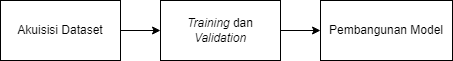
\includegraphics[scale=0.85]{gambar/metodologi_umum.png}
    \caption{Desain Sistem Keseluruhan}
    \label{fig:desainsistem}
\end{figure}

\section{Peralatan}
\label{sec:peralatan}
Peralatan yang digunakan pada penelitian ini yaitu Laptop. Laptop, digunakan pada keseluruhan implementasi metodologi ini. Adapun spesifikasi laptop yang digunakan pada penelitian ini adalah laptop dengan spesifikasi seperti pada tabel \ref{tb:spesifikasilaptop}.\par

\begin{table}[H]
    \begin{center}
        \begin{tabular}{|l|l|}
        \hline
        \textit{\textbf{Processor}}        & \begin{tabular}[c]{@{}l@{}}Intel Core i5-8300H \\ CPU @ 2.3 GHz (8 CPUs)\end{tabular} \\ \hline
        \textit{\textbf{Storage}}          & \begin{tabular}[c]{@{}l@{}}HDD 1 TB Storage\\ SSD 256 GB Storage\end{tabular}         \\ \hline
        \textit{\textbf{RAM}}              & \begin{tabular}[c]{@{}l@{}}16 GB SODIMM DDR4 \\ 2667 MHz Dual Channel\end{tabular}    \\ \hline
        \textit{\textbf{Graphic Card}}     & \begin{tabular}[c]{@{}l@{}}NVIDIA GeForce GTX 1050 Ti \\ 4 GB GDDR5\end{tabular}      \\ \hline
        \textit{\textbf{Operating System}} & \begin{tabular}[c]{@{}l@{}}Windows 10 Home \\ Single Language 64-bit\end{tabular}     \\ \hline
    \end{tabular}
    \caption{Spesifikasi Laptop yang Digunakan}
    \label{tb:spesifikasilaptop}
    \end{center}
\end{table}

\section{Desain Sistem}
\label{sec:desainsistem}

Tugas akhir ini merupakan penelitian dalam bidang visi komputer yang bertujuan untuk mendeteksi huruf balok tulisan tangan pada media papan tulis menggunakan metode \textit{you only look once} (YOLO). Adapun secara umum alur desain sistem yaitu seperti pada gambar \ref*{fig:desainsistem}. Perancangan model menggunakan metode YOLO, lebih spesifik yaitu YOLOv5. \par

Berdasarkan gambar \ref*{fig:desainsistem}, langkah awal yang harus dilakukan yaitu proses akuisisi dataset, yaitu dengan mengumpulkan data tulisan tangan huruf balok pada media papan tulis dan setelahnya juga dilakukan pre-proses tertentu yang akan dijelaskan pada sub akuisisi data. Proses selanjutnya yaitu dengan melakukan konfigurasi-konfigurasi pada model sebelum dilakukan training, dan ketika sudah dilakukan proses training maka hasil model yang telah dibuat tersebut dievaluasi dengan confusion matrix. \par

% Per blok diagram dijelaskan dan dibuatkan section masing-masing

\section{Akuisisi Dataset}
\label{sec:akuisisidataset}

Dalam pelaksanaan proses akuisisi dataset, terdapat beberapa bagian proses yang harus dilakukan yang dapat dilihat pada blok diagram berikut.

\begin{figure}[ht]
    \centering
    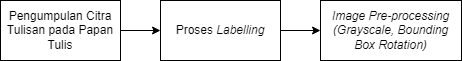
\includegraphics[scale=0.85]{gambar/metodologi_akuisisi_data.png}
    \caption{Alur Akuisisi Dataset}
    \label{fig:alurakuisisidataset}
\end{figure}

\subsection{Pengumpulan Citra Tulisan pada Papan Tulis}
\label{subsec:pengumpulancitra}

Proses pengumpulan citra huruf balok tulisan tangan pada papan tulis dimulai dengan menentukan jumlah kelas dataset yang akan digunakan. Pada huruf alfabet, terdapat 26 huruf dari A sampai Z yang artinya pada proses akuisisi dataset ini nantinya akan terdapat 26 kelas yang mewakili masing-masing huruf tersebut. Setelah jumlah kelas ditentukan, proses selanjutnya yaitu membuat huruf balok tulisan tangan pada media papan tulis kemudian mengambil gambar dari huruf balok tulisan tangan tersebut. Proses tersebut diulang sebanyak beberapa kali pada tiap kelas yang sama dan diulang kembali sesuai jumlah kelas yang tersedia. \par

\subsection{Proses Pelabelan Dataset}
\label{subsec:proseslabelling}

Proses pelabelan yaitu merupakan proses pemberian label dengan memberikan \textit{bounding box} pada objek dan nama kelas pada objek tersebut. Tujuan dari proses pelabelan ini yaitu untuk mendapatkan \textit{ground-truth bounding box}. Proses pelabelan dilakukan dengan menggunakan bantuan \textit{tool} yaitu Roboflow, dan dilihat pada gambar \ref*{fig:labellingroboflow}. Sebelum proses pelabelan dilakukan, citra yang telah dikumpulkan sebelumnya diupload pada \textit{workspace} Roboflow. Setelah diberikan \textit{bounding box}, citra yang telah diberikan label selanjutnya dibagi menjadi \textit{training sets} dan \textit{testing sets}. Adapun pembagian \textit{training testing sets} menggunakan komposisi 80\% \textit{training sets} dan 20\% \textit{testing sets}. \par

\begin{figure}[H]
    \centering
    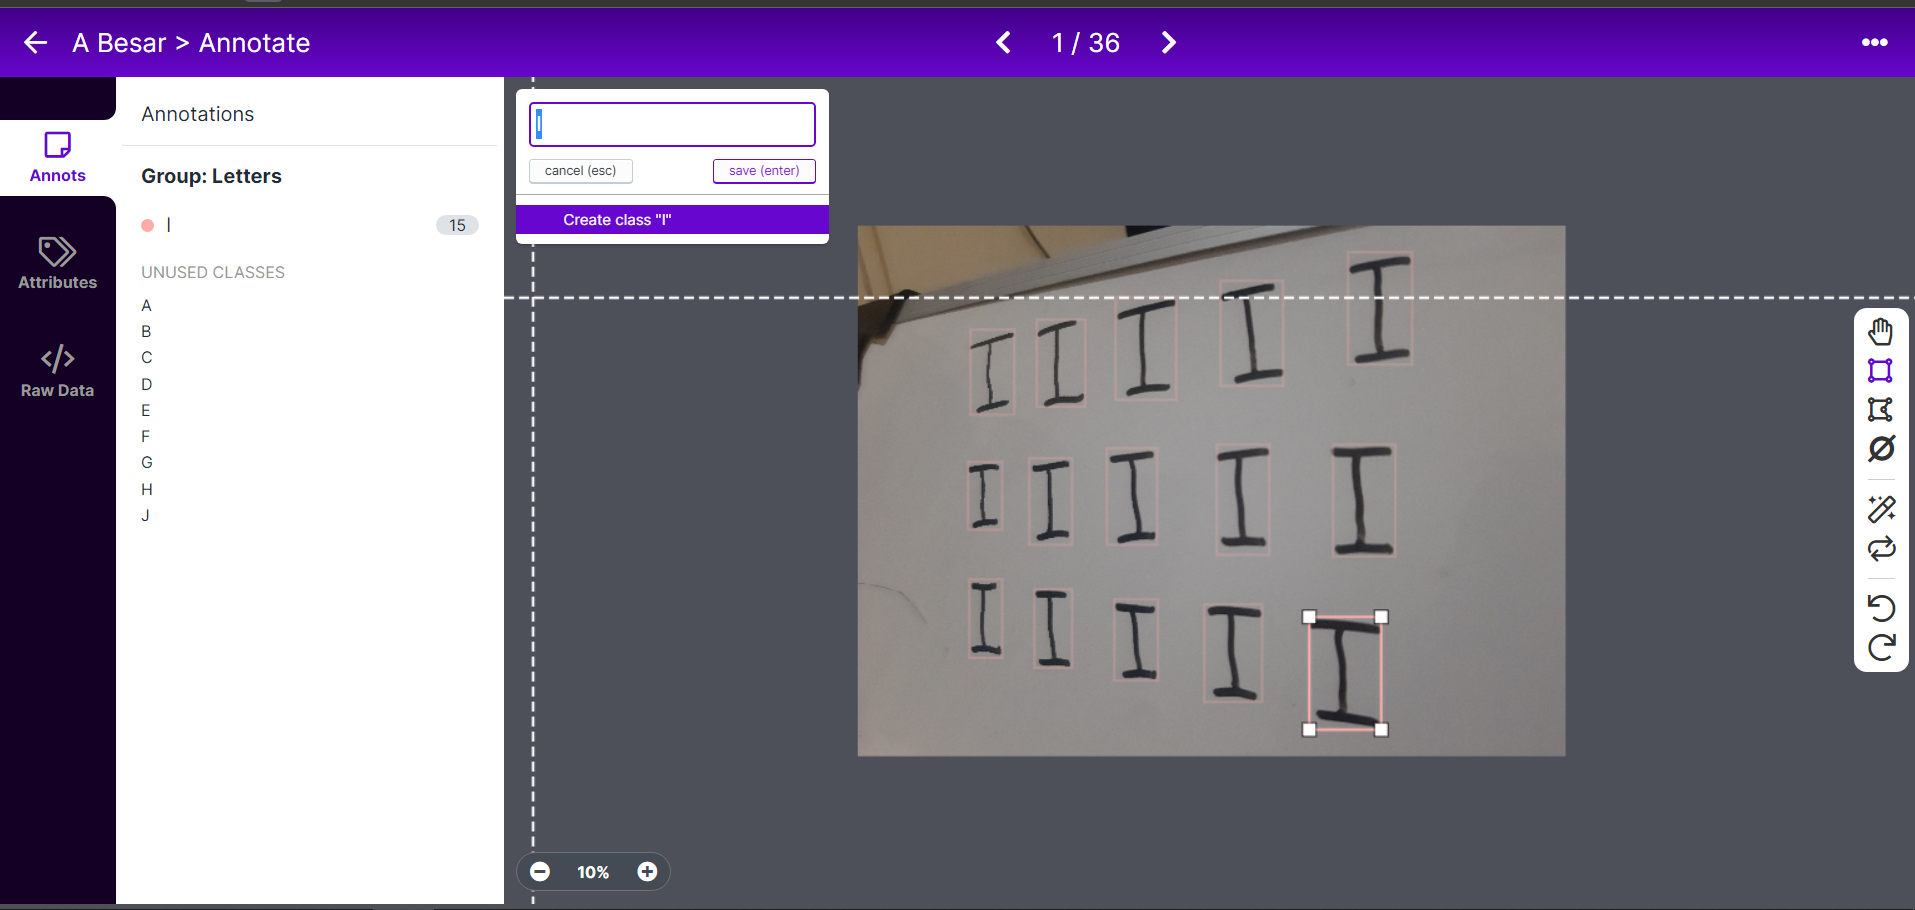
\includegraphics[scale=0.25]{gambar/labelling.png}
    \caption{Proses Pelabelan menggunakan Roboflow}
    \label{fig:labellingroboflow}
\end{figure}

\subsection{\textit{Image Pre-Processing}}
\label{subsec:imagepreprocess}

Pada tahapan \textit{image pre-processing} ini dilakukan 3 jenis pre-proses yaitu \textit{resize, grayscalling}, dan \textit{bounding box rotation}. Pada proses \textit{resize}, citra yang telah diambil ukurannya diperkecil (diregangkan) menjadi ukuran 416x4 16, hal ini bertujuan untuk memperkecil ukuran file serta mempercepat proses \textit{training} mengingat jumlah data dan jumlah kelas yang sangat banyak. \par

\begin{figure}[H]
    \centering
    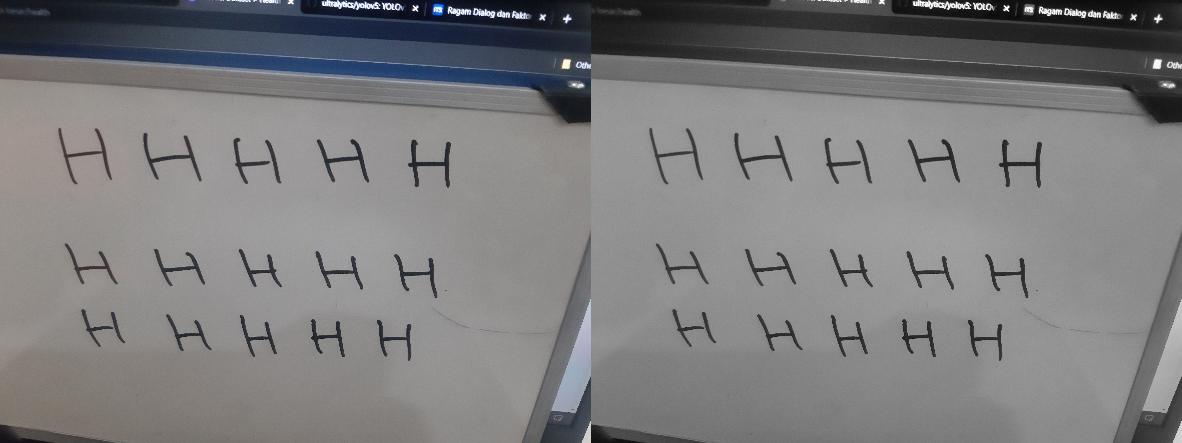
\includegraphics[scale=0.35]{gambar/grayscalling.png}
    \caption{Gambar Sebelum dan Setelah Proses \textit{Grayscalling}}
    \label{fig:grayscallingdataset}
\end{figure}

Pada proses \textit{grayscalling}, gambar dibuat menjadi warna abu dengan tujuan untuk memperkecil variasi warna spidol pada media papan tulis sehingga model yang dibuat berfokus hanya pada pola tulisan tangan pada papan tulis saja dan tidak terfokus ke warna yang digunakan untuk menulis pada papan tulisnya. \par

\begin{figure}[H]
    \centering
    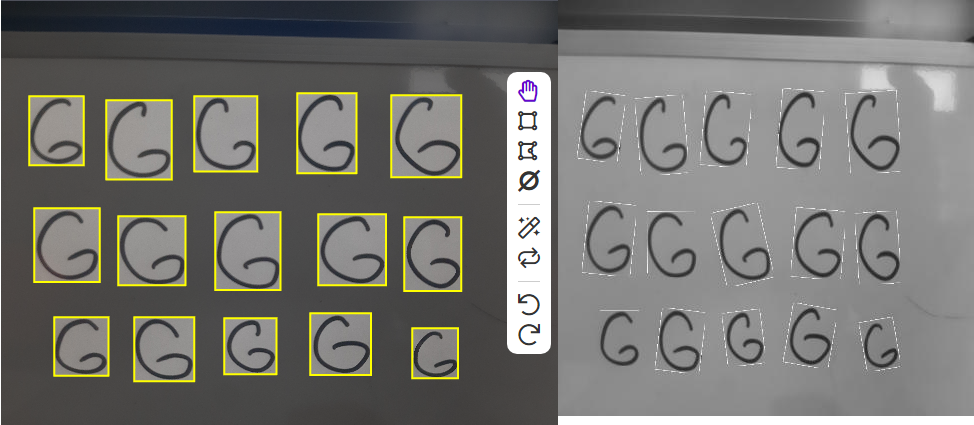
\includegraphics[scale=0.32]{gambar/bbrotation.png}
    \caption{Gambar Sebelum dan Setelah Proses \textit{Bounding Box Rotation}}
    \label{fig:bbrotation}
\end{figure}

Terakhir, dilakukan proses \textit{bounding box rotation} seperti pada gambar \ref*{fig:bbrotation}, yaitu melakukan rotasi pada skala \textit{bounding box}, tujuannya untuk menambah variasi sehingga model yang tercipta lebih akurat ketika pengambilan citra tidak diambil tepat didepan objek. Adapun konfigurasi dari \textit{bounding box rotation} yaitu antara -15\textdegree\space dan +15\textdegree. \par
% perlu g y tabel konfigurasi preproses yang digunakan

\section{Training}
\label{sec:trainingdata}

\textit{Training data} dilakukan setelah proses pengumpulan citra, proses pelabelan, dan pre-proses gambar selesai dilaksanakan. Dalam proses \textit{training}, dibutuhkan konfigurasi \textit{hyperparameter} tertentu seperti jumlah epochs, \textit{batch size}, dan jenis \textit{pretrained weight} yang akan digunakan. Pada tugas akhir ini, versi YOLO yang digunakan yaitu YOLOv5. \par

Sebelum proses \textit{training} dilakukan, perlu ditentukan jenis \textit{pretrained weights} yang akan digunakan. Pada YOLOv5, terdapat beberapa jenis \textit{pretrained weights} yang tersedia yaitu YOLOv5n, YOLOv5s, YOLOv5m, YOLOv5l, dan YOLOv5x. Pada tugas akhir ini, \textit{pretrained weight} yang digunakan yaitu YOLOv5s. \par
% Adapun konfigurasi layer YOLOv5 secara lebih lengkap telah dibahas pada tinjauan pustaka ttg yolov5 

Setelah menentukan jenis \textit{pretrained weight} yang akan digunakan, selanjutnya yaitu menentukan konfigurasi \textit{hyperparameter} untuk data yang akan di-\textit{train}. Konfigurasi \textit{hyperparameter} yang dilakukan yaitu pengaturan epochs, \textit{batch size,} dan \textit{image size}. \par

\begin{table}[H]
    \begin{center}
        \begin{tabular}{|l|c|}
        \hline
        \multicolumn{1}{|c|}{\textbf{Parameter}} & \textbf{Nilai} \\ \hline
        \textit{Weights}                         & YOLOv5s                 \\ \hline
        Epochs                                   & 30                      \\ \hline
        \textit{Batch-Size}                      & 16                      \\ \hline
        \textit{Image Size}                      & 416                     \\ \hline
        \end{tabular}
    \end{center}
    \caption{Detail Parameter yang Digunakan}
    \label{tb:parametertrain}
    \end{table}

\noindent Adapun penjelasan dari masing-masing pengaturan yaitu: \par
\begin{enumerate}[nolistsep]
    \item \textbf{Epochs}. Epochs adalah \textit{hyperparameter} yang berfungsi untuk menentukan jumlah pengulangan atau berapa kali suatu algoritma \textit{learning} akan melakukan proses \textit{learning} suatu \textit{dataset training}. Secara sederhana, semakin besar jumlah epochs maka model yang dihasilkan memiliki tingkat akurasi yang lebih tinggi namun waktu yang dibutuhkan untuk melakukan \textit{learning} akan semakin lambat. Pada tugas akhir ini, epochs yang digunakan yaitu 30.
    \item \textit{\textbf{Batch-size}}. \textit{Batch-size} adalah \textit{hyperparameter} yang berfungsi untuk mengontrol jumlah sampel training untuk dikerjakan sebelum parameter internal model diperbarui. Pada tugas akhir ini, \textit{batch-size} yang digunakan yaitu 16.
    \item \textit{\textbf{Image Size}}. \textit{Image size} adalah ukuran gambar yang diterapkan pada \textit{dataset}. Pada tugas akhir ini, \textit{dataset} menggunakan \textit{image size} berukuran 416x416.
\end{enumerate}
% tambahkan tabel spesifikasi model yg digunakan

\section{Hasil Model}
\label{sec:hasilmodel}

Pada tahapan hasil model, setelah dilakukan proses \textit{training,} hasil tersebut akan tersimpan pada direktori 'runs/train/..'. Pada direktori tersebut didapatkan \textit{checkpoint} hasil model beserta dengan grafik atau detil data hasil pada tiap proses pengulangan. \par
% tampilkan gambar result.csv
% tampilkan hasil deteksi

Pada tahapan selanjutnya, ketika hasil model dirasa telah cukup bagus baik itu dari segi data angka performa maupun dari hasil proses deteksi, selanjutnya yaitu pembuatan algoritma konversi gambar menjadi teks. Proses penyusunan teks dimulai dari menentukan koordinat seluruh \textit{bounding box} yang tersedia. Setelah koordinat \textit{bounding box} didapat, seluruh \textit{bounding box} yang terbaca dikelompokan berdasarkan kedekatan antara \textit{bounding box} pertama dengan \textit{bounding box} selanjutnya, jika jarak antaranya memenuhi \textit{threshold} tertentu maka akan dikelompokan menjadi 1, dan jika tidak memenuhi maka akan diletakan pada kelompok berikutnya. Adapun prioritas pengelompokan diatur berdasarkan koordinat Y dahulu lalu dilanjutkan dengan koordinat X, hal ini bertujuan agar teks yang ditampilkan berurutan dari baris atas lalu bergerak kearah X+, dan dilanjut pada baris kedua dan seterusnya. Alur dari pembentukan algoritma konversi gambar menjadi teks dapat dilihat pada gambar berikut. \par
% tampilkan flowchart pembuatan  
